\procTitle{Из истории научного кольцевания птиц Охотско-Колымского края}
\procAuthor{Юсупова~Е.\,А.}
\procEmail{yusupova.ea@magadanmuseum.ru}
\procOrganization{МОКМ} \procCity{Магадан}

\makeProcTitle
\index{x@Юсупова~Е.\,А.}

Кольцевание представляет собой один из наиболее эффективных методов изучения биологии птиц. С~помощью кольцевания возможно точное выяснение ряда важнейших научных и~практических вопросов, таких как определение направлений и~путей осенних и~весенних миграций птиц, мест зимовок и~гнездований, каким порядком расселяется молодняк и~расширяет гнездовую область, возраст гнездования, как изменяется оперение с~возрастом, сроки жизни разных видов, где, главным образом, гибнут перелётные птицы во время миграций и~многие другие вопросы. [2, С.~39]

В\ \ Советском\ \ Союзе\ \ массовое\ \ кольцевание\ \ птиц было организовано с~1924~г. на Биостанции Юных Натуралистов в~Москве, в~Сокольниках. Вообще в~истории развития кольцевания птиц в~СССР большую роль сыграли юные натуралисты. По их инициативе возникло это дело в~нашей стране. Юные натуралисты, или юннаты, своей работой заложили краеугольный камень массовых орнитологических исследований. Вот почему первые годы на кольцах кроме надписи Moskwa, номера и~серии стояла ещё аббревиатура <<БЮН>> (Бюро юных натуралистов).

\begin{wrapfigure}{r}{6cm}
%\begin{changemargin}{-1.5cm}{0cm}
    \begin{center}
    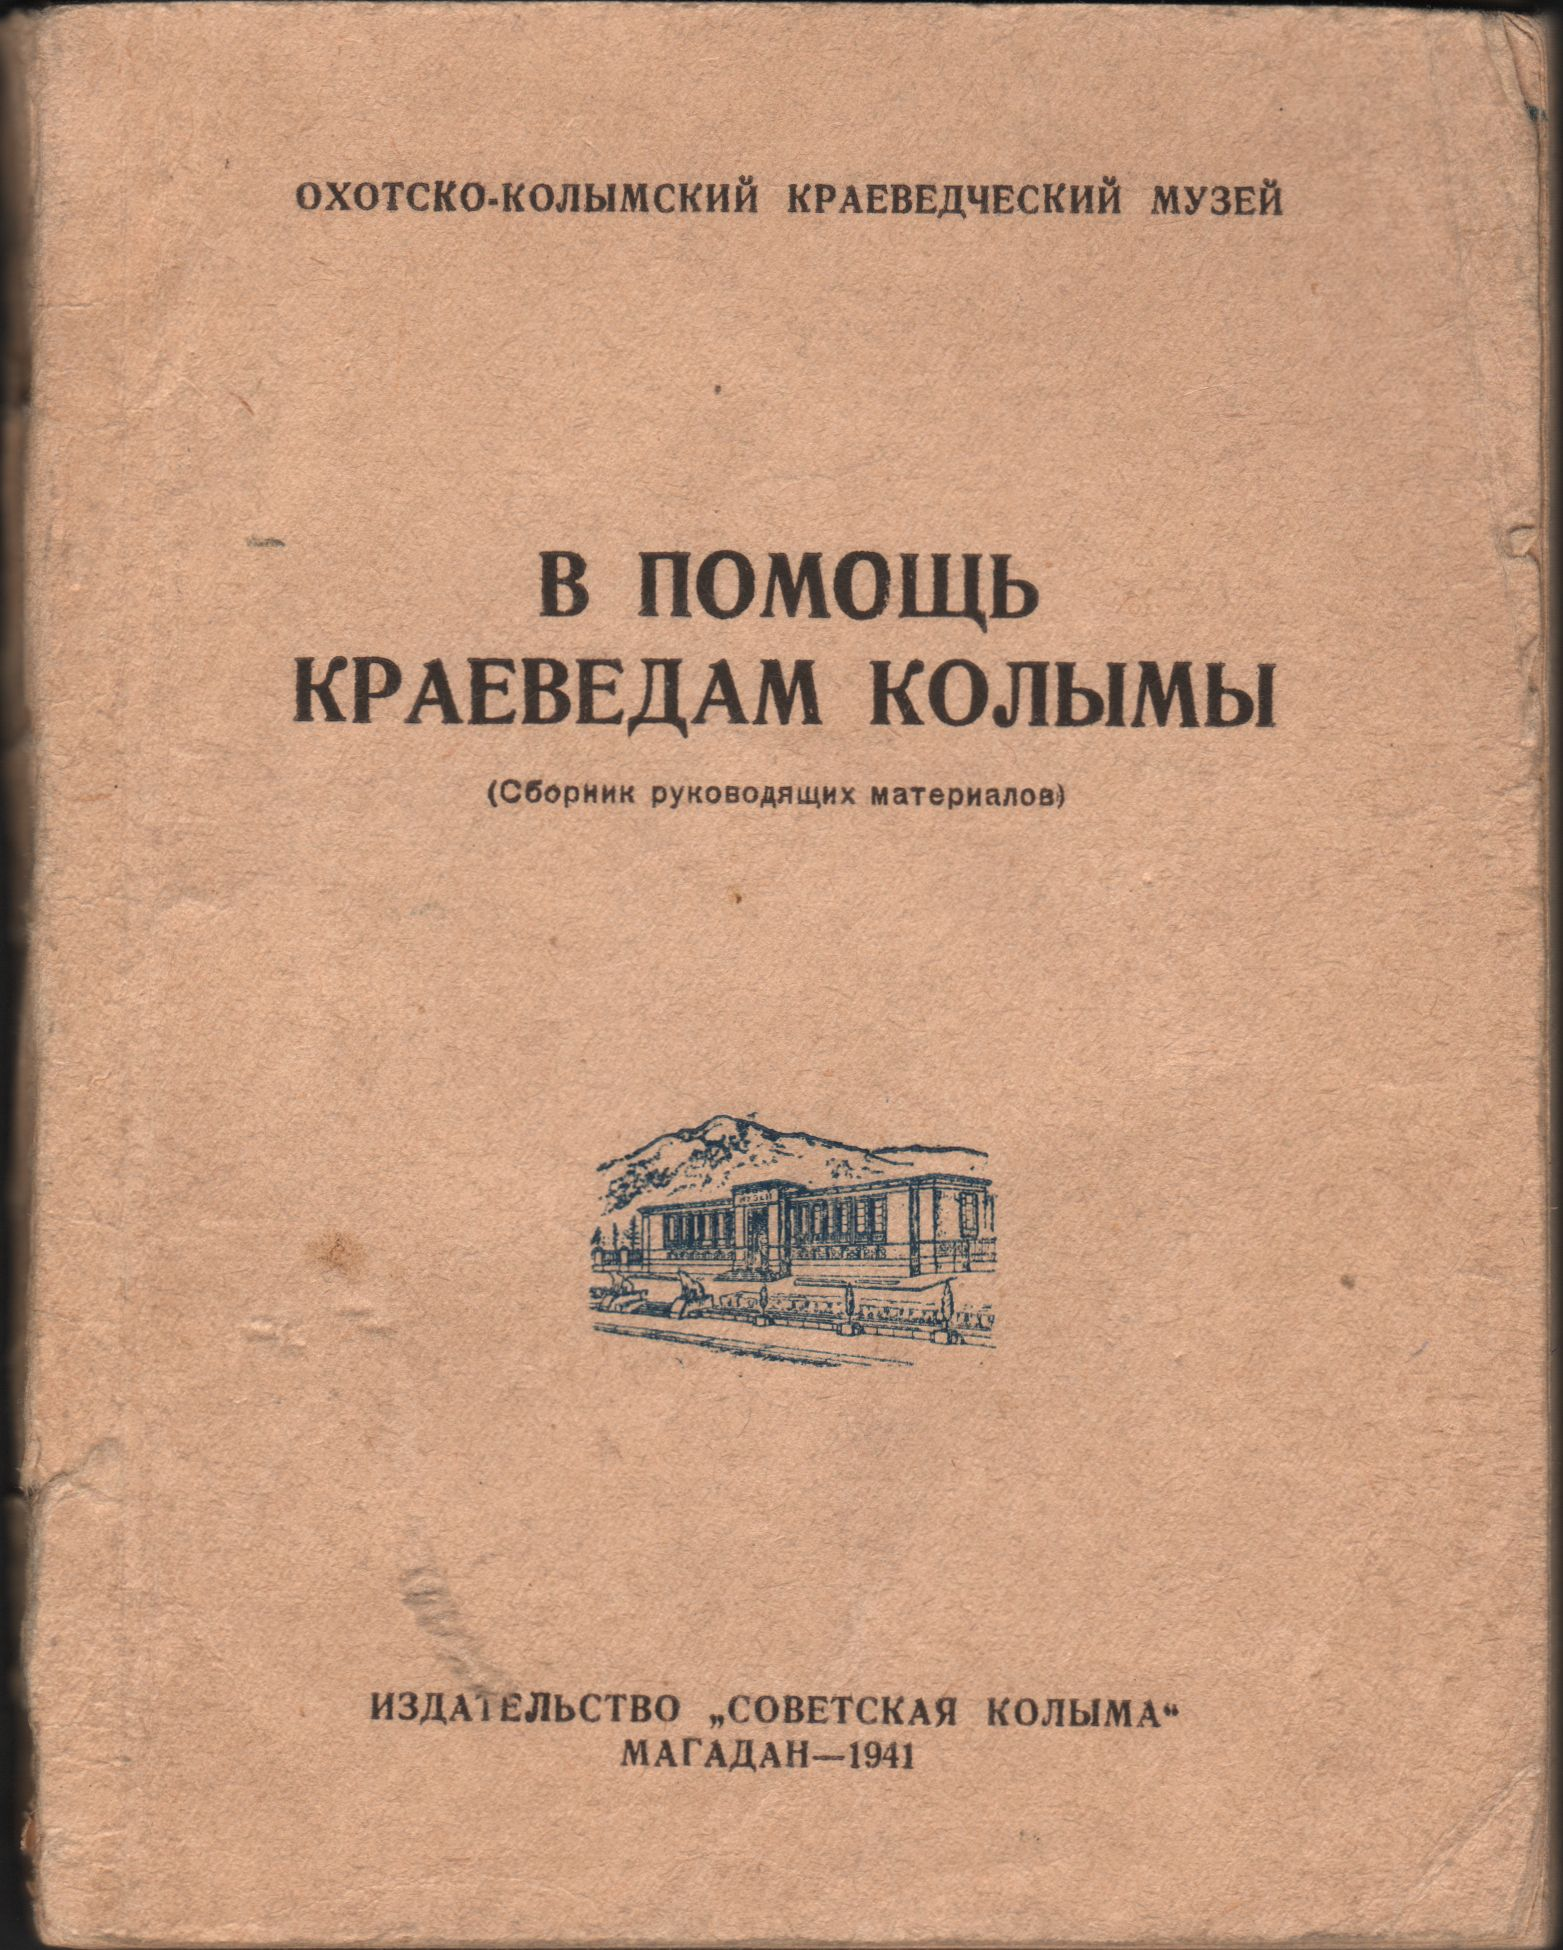
\includegraphics[width=0.4\textwidth]{authors/usupova-fig-1.jpg}
  \end{center}
  \caption{Брошюра <<В помощь краеведам Колымы. Сборник руководящих материалов>> [6]}
  \label{fig:usupova-fig-1}
%  \end{changemargin}
\end{wrapfigure}


Недавно сложившееся собрание орнитологических колец Магаданского областного краеведческого музея насчитывает 11 единиц, начиная с~экземпляров 30-х гг. ХХ~в. и~заканчивая современными образцами.

Магадан обрёл статус города в~1939~г. В то время центром научно-исследовательской и~просветительской работы в~Магадане был Охотско-Колымский краеведческий музей, который находился в~ведении ад\-ми\-нист\-ра\-тив\-но-гражданского отдела Дальстроя [3, С.~20]. Гораздо позже нишу научных изысканий прочно заняли такие исследовательские институты, как СВКНИИ ДВО РАН (1960~г.) и~ИБПС ДВО РАН (1972~г.). В фондах, архиве и~библиотеке музея имеется большое количество литературы (книги, брошюры, отчёты об экспедициях), подтверждающей обширную научную работу музея в~первые десятилетия основания города.

В книжном фонде музея имеется брошюра 1941~г. <<В помощь краеведам Колымы. Сборник руководящих материалов>> (рис.~1), изданная по инициативе А.~П.~Хмелинина, неутомимого популяризатора краеведческих знаний. Видное место в~сборнике занимает статья <<О кольцевании птиц>>. Основная цель работы по кольцеванию птиц, отмеченная в~данной статье – выяснение миграционных путей перелётных птиц и~их гнездовых ареалов, сроков жизни различных видов, осенних и~зимних кочёвок и~других аспектов жизни птиц. Также в~статье чётко обозначена роль Охотско-Колымского музея как консультационного центра по вопросам кольцевания птиц и~<<связующего звена>> с~Центром кольцевания птиц в~Москве.

На тот момент на Дальнем Востоке и~в~нашем крае имелись огромные запасы промысловой птицы, слабо использующиеся. Между тем знание путей перелетов, мест зимовок и~гнездовий этих видов позволило бы правильно вести отстрел и~охрану промысловой дичи, правильно организовать охотничье хозяйство. Массовая работа по кольцеванию птиц среди охотников, колхозников, краеведов, а также учеников школ должна была дать большой эффект по изучению биологических аспектов ценных для хозяйства видов птиц. Надо отметить, что при общем малом количестве находок окольцованных птиц и~возвратов меточных колец наибольший процент возвратов всегда давали именно охотничье-промысловые виды птиц. Например, если в~книге С.~А.~Бутурлина 1948~г. указанная доля возвратов равна 6\,\% [1, С.~32], то в~<<Инструкции по кольцеванию птиц>> 1952~г. это число равно 5\,\%.  [4, С.~5]

Охотничье-промысловыми видами птиц считались утки, гуси, океанические птицы (в прибрежных районах). Из боровой дичи большое значение имели куропатка, глухарь, рябчик [8, С.~468]. Для кольцевания значительный интерес представляют также птицы, живущие колониями – например, чайка. Рекомендуется кольцевать и~таких птиц, как кукша, кедровка, ворон [2, С.~40].

Проводимая грандиозная работа по превращению края в~промышленный район требовала всестороннего изучения края. Эта почётная задача была поставлена перед музеем. С~12~июня по~1~сентября 1939~г. прошла экспедиция по маршруту <<Магадан~--- устье р.~Колымы>>. Это была первая краеведческая экспедиция, организованная музеем. Она имела рекогносцировочное значение, в~том числе целью экспедиции был сбор коллекций по флоре и~фауне бассейна р. Колымы [6, С.~3].

Во время экспедиции музей организовал несколько краеведческих кружков и~выдал населению меточные кольца и~инструкции по кольцеванию птиц и~сбору материала. В <<Отчете о краеведческой экспедиции музея\dots>> (рис.~2) перечислены номера 24~колец, выданных музеем на местах. Из них 5~колец выданы на Среднеканскую метеостанцию Борису Александровичу Александрову (№№ колец 9520, 9519, 37272, 37264, 37263), 9 колец~--- Михаилу Алексеевичу Куштысеву, руководителю Коркодонского краеведческого кружка (№№ колец 9517, 37270, 9518, 37260, 37265, 9530, 37287, 37279, 37283), и~10 колец~--- Владимиру Афанасьевичу Ковалеву, руководителю краеведческого кружка Нагаево (№№ колец 9523, 9521, 9532, 37289, 37291, 37282, 37290, 37275, 37284, 37276) [6, С.~8--9, 19,37]. К сожалению, выяснить дальнейшую судьбу этих колец не удалось.

\begin{figure}[H]
  \begin{center}
    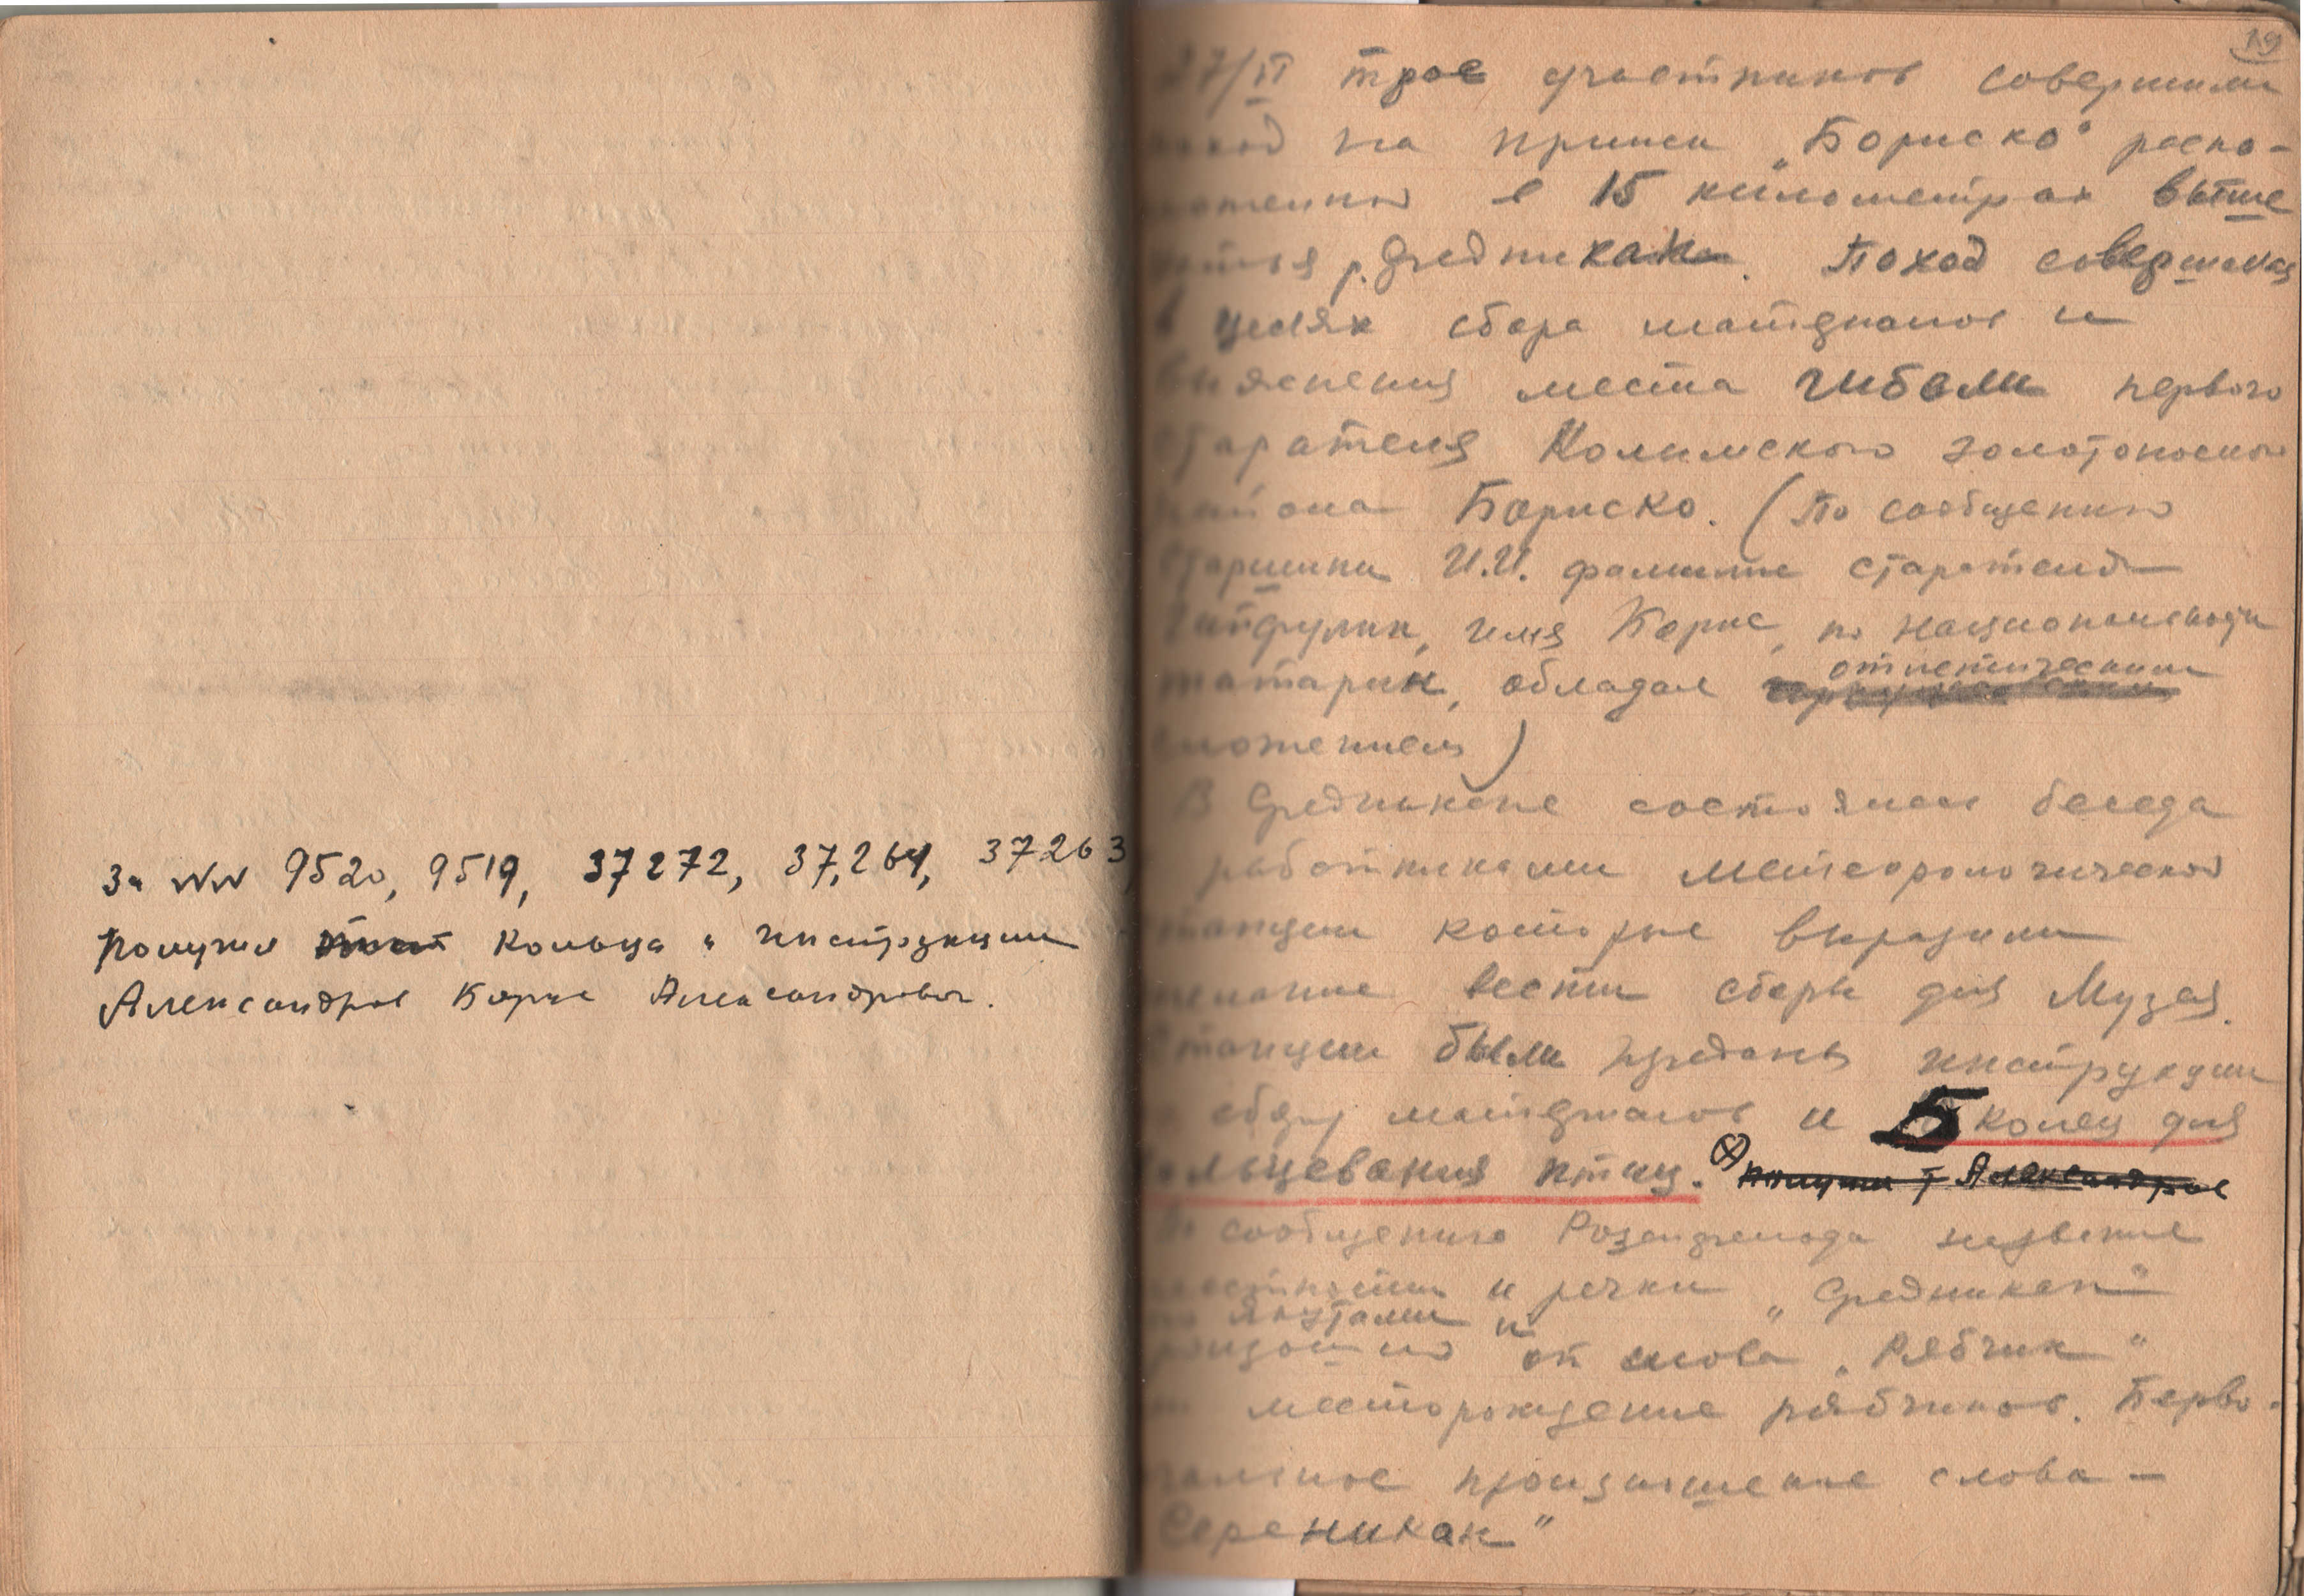
\includegraphics[width=1\textwidth]{authors/usupova-fig-2.jpg}
  \end{center}
  \caption{Страница из отчёта о краеведческой экспедиции музея по маршруту Магадан~--- устье р.~Колыма, 1939~г. [7]}
  \label{fig:usupova-fig-2}
  \vspace{-8pt}
\end{figure}


Сотрудник Центра кольцевания птиц Ирина Харитонова пояснила, что для работы необходимо знать буквенные серии колец. В экспедиционном отчёте же перечислены только цифры. Кольца с~одними только номерами появились не раньше конца 1970-х гг., а до этого перед номером (иногда после него) ставилась определённая буква. В качестве примера можно привести размерные группы колец, отмеченные в~брошюре <<Инструкция по кольцеванию птиц>> 1952~г. выпуска.

\begin{description}[noitemsep]\vspace{-10pt}
\item[Серия <<А>>]~--- для самых крупных птиц: орлов, лебедей, пеликанов, аистов, журавлей;
\item[Серия <<В>>]~--- для гусей, глухарей, крупных хищников;
\item[Серия <<С>>]~--- для крупных чаек, крупных уток и~хищников средней величины;
\item[Серия <<D>>]~--- для уток: кряквы, шилохвости, свиязи и~т.\,п., чаек средней величины, кайр, гагарок, тетеревов, грачей, ворон;
\item[Серия <<Е>>]~--- для мелких уток, куропаток, мелких хищников: пустельги, кобчика, ястреба – перепелятника;

\item[Серия <<F>>]~--- для перепелов, куликов, скворцов, дроздов;
\item[Серия <<G>>]~--- (без обозначения буквы на кольце)~--- для мелких воробьиных птиц. [4, С.~6]
\end{description}\vspace{-8pt}

\begin{wrapfigure}{r}{5cm}
%\begin{changemargin}{-1.5cm}{0cm}
    \begin{center}
    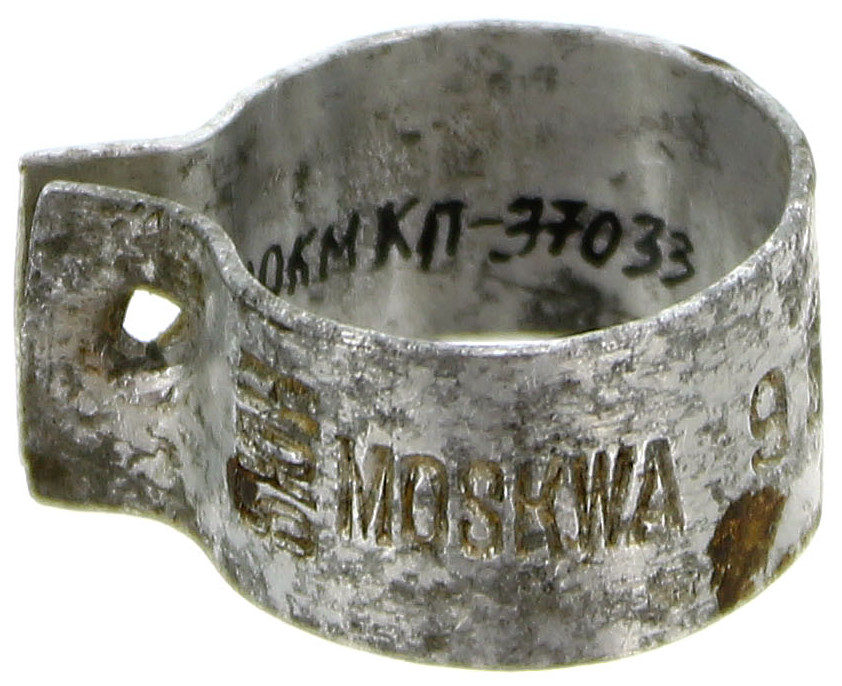
\includegraphics[width=0.35\textwidth]{authors/usupova-fig-3.jpg}
  \end{center}
  \caption{Кольцо орнитологическое для кольцевания, серия <<В>> <<БЮН MOSKWA 9506 В>> (Фонды МОКМ).}
  \label{fig:usupova-fig-3}
%  \end{changemargin}
\end{wrapfigure}


В 2019~г. при пересмотре предметов из старых поступлений было обнаружено кольцо для мечения птиц с~шифром <<БЮН MOSKWA 9506~B>> (рис.~3). Хранитель музейной коллекции <<Естественно-исторические материалы>> обратилась в~Центр кольцевания птиц России с~просьбой выяснить историю кольца, для этого она указала его шифр. В ответ на письмо пришла следующая информация: <<\textit{\dotsкольцо было выдано Краеведческому музею~г. Магадан в~1946 или 1947~г. Теоретически, это кольцо могло остаться у кольцевателей и~не быть использованным}>>.
\clearpage

Из\ \ этого\ \ следует, что,\ \ возможно,\ \ кольцо было заказано у Центра А.~П.~Хмелининым для дальнейшей научно-исследовательской работы, но так и~не было использовано. В 1946~г. А.~П.~Хмелинин настойчиво инициировал создание заповедника на полуострове Кони, фактически став одним из его основателей. Для выполнения задуманного, он отдавал все свободное от службы время подготовке материалов с~обоснованием необходимости создания заповедника в~Ольский районный Совет депутатов трудящихся. От~решения организационных вопросов директор музея во второй половине 1940-х~гг. перешёл к изучению территории будущего заповедника в~ходе различных экспедиций [5, С.~178]. С июня по сентябрь 1948 года музей проводил летнее обследование полуострова Кони. В частности, сотрудников музея интересовали редкие виды птиц и~животных. Автор отчёта Мощенко~Ю.~К. отмечает, что кольцевание птиц он не производил ввиду невозможности добывания птиц. Из 50 колец, взятых им в~экспедицию, было израсходовано только одно. Этим кольцом 15 ноября*\footnote{*~--- Возможно, описка.  Даты экспедиции обозначены в~тексте <<с 17/ VI 1948~г. до~20~сент. 1948~г.>>, а дата кольцевания тулеса указана в~тексте <<15го XI~--- 48~г.>>.} 1948~г. в~посёлке Умара на северном побережье полуострова Кони был окольцован тулес. Указан и~номер кольца: 37237 серия <<D>> [7, С.~68]. Вероятно, упомянутое выше кольцо с~аббревиатурой <<БЮН>> входило в~число этих 50 колец и~предназначалось для работы на территории будущего заповедника. Именно оно и~положило начало музейному собранию орнитологических колец.

\begin{thebibliography}{99}

\bibitem{}\BibAuthor{Бутурлин~С.~А.} Что и как наблюдать в жизни птиц.~--- М.~: Изд-во московского общества испытателей природы, 1948.~--- 126~с.
\bibitem{}В помощь краеведам Колымы. Сборник руководящих материалов.~--- Магадан~: <<Советская Колыма>>, 1941.~--- 89~с.~--- Фонд МОКМ.
\bibitem{}Заповедник <<Магаданский>>. Фотоальбом.~--- М.~: <<ПЕНТА>>, 2012.~--- 104~с.
\bibitem{}Инструкция по кольцеванию птиц.~--- М.~: Загорская типография, 1952.~--- 16~с.
\bibitem{}Новатор Колымского края (Первый естествоиспытатель Северо-Востока СССР А.~П.~Хмелинин) // Исторические, философские, политические и юридические науки, культурология и искусствоведение. Вопросы теории и практики: научно-теоретический и прикладной журнал: scientific-theoretical and applied journal.~--- 2017.~--- Ч.~1, №~10 (84).~--- С.~175--180.
\bibitem{}Отчет о краеведческой экспедиции музея по маршруту <<Магадан~--- устье р.~Колымы>>, 1939~г.~--- Научный архив МОКМ.
\bibitem{}Отчет сотрудника Охотско-Колымского краеведческого музея тов. Мощенко~Ю.~К. о~летнем обследовании полуострва Кони, 1948~г.~--- Научный архив МОКМ.
\bibitem{}\BibAuthor{Сергеев~М.~А.} Народное хозяйство Камчатского края.~--- М.--Л.~: Изд-во АН~СССР, 1936.~--- 815~с.



\end{thebibliography}
